% !TeX program = xelatex
\documentclass[UTF8,fontset=none,11pt,a4paper]{ctexart}
\usepackage{fontspec}
\setmainfont{TeXGyreTermes}
\setCJKmainfont[BoldFont={Noto Serif CJK SC Bold}]{Noto Serif CJK SC}
\setCJKsansfont{Noto Sans CJK SC}
\usepackage{geometry,graphicx,amsmath,amssymb,booktabs,xcolor,fancyhdr,hyperref}
\geometry{left=22mm,right=22mm,top=22mm,bottom=21mm,headheight=15pt}
\definecolor{deep}{HTML}{164960}
\pagestyle{fancy}\fancyhf{}\fancyhead[L]{\small Hyser / Hard HiWA 实验}\fancyhead[R]{\small 2026.11.17}\fancyfoot[C]{\thepage}
\setlength{\parindent}{2em}\setlength{\parskip}{6pt}
\newcommand{\plotpage}[3]{\clearpage\section{#1}
\begin{center}\includegraphics[width=.98\textwidth,height=.72\textheight,keepaspectratio]{figures/#2}\end{center}
\noindent\small #3\normalsize}
\begin{document}
\begin{center}
{\huge\bfseries\color{deep}真实 Hyser 数据的 Hard HiWA 对齐实验}\\[5pt]
{\large 仅源域 K-means，目标域继承同步组标签}\\[6pt]
250 对同步窗口；三维白化；二维/三维散点对比
\end{center}
\section{数据、预处理与唯一分组}
PhysioNet Hyser Random Task，subject01/session1/sample1，长25秒。
肌电 256 通道、2048Hz；手指力量5通道、100Hz。
每0.1秒取一个同步窗口（共250对）。肌电经通道RMS、log1p、Z-score、PCA降至三维；
力量取拇指、中指、食指的三维窗口平均值。两域分别做协方差白化：
\[
\widetilde X=(X-\bar X)\Sigma_X^{-1/2},\quad
\widetilde Y=(Y-\bar Y)\Sigma_Y^{-1/2},\quad
\operatorname{Cov}(\widetilde X)\simeq\operatorname{Cov}(\widetilde Y)\simeq I_3.
\]
只在源域做一次K-means（$K=4$、seed42、初始化次数30），组大小为46、53、91、60；
目标域按照同步窗口一一继承相同组标签，绝不单独聚类。传递组标签使用了真实配对，
因此它是\textbf{已知组对应的诊断实验，而不是完全无监督HiWA}。

\section{全量对齐误差}
令$E=\widetilde XR^\top-\widetilde Y$，平方误差$SSE=\|E\|_F^2$。
\[
R^2=1-\frac{SSE}{\|\widetilde Y-\overline{\widetilde Y}\|_F^2},\quad
\mathrm{rSE}=\frac{SSE}{\|\widetilde Y\|_F^2},\quad
\overline{d}=\frac1{250}\sum_{i=1}^{250}\|E_i\|_2.
\]
\begin{center}
\begin{tabular}{lrrr}
\toprule
方法 & $R^2\uparrow$ & $\mathrm{rSE}\downarrow$ & $\overline d\downarrow$\\
\midrule
对齐前 & $-0.6741$ & 1.6741 & 1.9775\\
自由簇级OT的Hard HiWA & $-0.1691$ & 1.1691 & 1.6977\\
固定已知簇对应的HiWA变体 & $-0.1539$ & 1.1539 & 1.6880\\
使用真实配对的最佳正交Oracle & $-0.1369$ & 1.1369 & 1.6884\\
\bottomrule
\end{tabular}
\end{center}
这里两个域均已白化，尺度处理已经统一。Oracle使用真实逐点配对计算，因此只作为正交模型的理论参照。

\plotpage{对齐前：源域唯一K-means，目标域继承标签}{01_before_hiwa.png}{
上排为三维，下排为二维；左列为目标域，右列为源域。两边同色代表同一组真实同步窗口，不存在目标域独立聚类。}

\plotpage{自由簇级OT：Hard HiWA对齐后}{02_after_hiwa_free.png}{
使用原版允许自由簇匹配的HiWA结构，μ=0.005；第75轮停止，旋转变化0.0802，但局部共识残差0.9899，不能认为严格ADMM收敛。}

\plotpage{固定已知组对应：Hard HiWA变体对齐后}{03_after_hiwa_fixed.png}{
将组级传输强制为$P=I_4/4$，仅优化对应簇对，μ=0.05。
60轮后旋转变化0.003389、局部共识残差0.005505，均低于0.01。
本方法额外使用组级监督约束，不是原版自由组HiWA。}

\clearpage
\section{Oracle、数值限制和结论}
最佳正交矩阵使用真实配对计算：
\[
R_*=\mathop{\arg\min}_{R^\top R=I_3}\|\widetilde XR^\top-\widetilde Y\|_F^2,
\quad \widetilde Y^\top\widetilde X=U\Sigma V^\top,\quad R_*=UV^\top.
\]
Oracle最小化总平方误差，而不一定最小化平均欧氏距离，
故固定组方法的平均距离可以略低于Oracle的平均距离。
尽管白化使均值、协方差一致，生理时滞、噪声、非线性等仍可能造成样本几何不相容。
自由簇和固定簇版本还使用不同$\mu$，不能将结果差别归因于固定$P$本身。
\begin{center}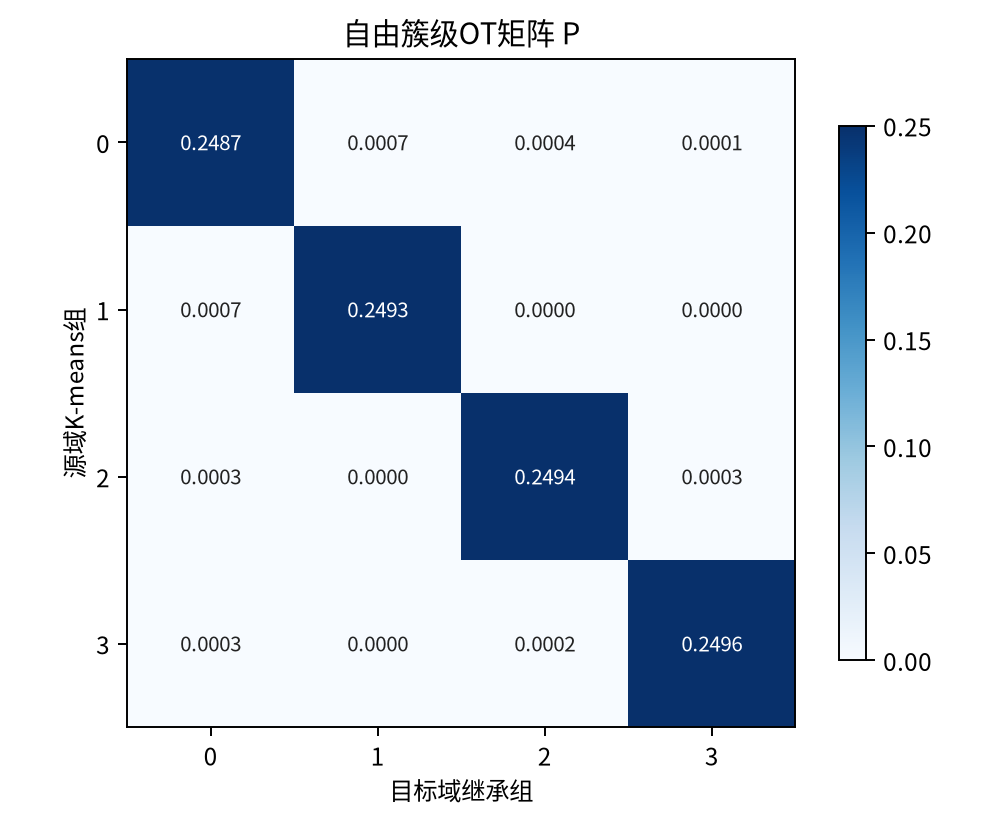
\includegraphics[width=.7\textwidth,height=.30\textheight,keepaspectratio]{figures/04_free_group_transport.png}\end{center}
\noindent\small 数值来自真实Hyser点云上按用户上传的GCOT/HiWA核心更新公式手工移植的本地求解器，
而非直接导入远程源文件。全部250点用于拟合内评价，
且同步关系被用于传递组标签，因此不是无监督算法的严格性能对比。\normalsize

\clearpage
\section{补充：源域软分组与继承隶属度}
为了只检验分组软化的作用，本轮保留250对真实白化三维数据，目标域仍继承源域的同步组信息，
只是把原本的$A_{ik}\in\{0,1\}$改为概率$A_{ik}\in(0,1)$，
并令$B_{ik}=A_{ik}$。目标域从始至终\textbf{不再独立聚类}。

一方面，固定源域K-means簇中心并软化距离：
\[
 A_{ik}\propto\exp\left(-\|x_i-c_k\|_2^2/\tau\right),\qquad \tau=0.5.
\]
另一方面，采用新GCOT代码的原型优化公式（只在源域学习）：
\[
 \min_C\|AC-X\|_F^2+
 \frac{\lambda_h}{N}\sum_{ik}A_{ik}\log A_{ik},\qquad
 A=\operatorname{softmax}(XC^\top),\quad\lambda_h=1.
\]
两个软模型均把同一个$A_i$传给目标域的同步窗口。
这属于\textbf{已知组对应的Soft-GCOT式诊断变体}，
不同于原论文在两域分别估计软分组的无监督GCOT。

固定$P=I_4/4$，共同使用$\mu=0.05$、样本熵正则$\varepsilon_s=0.1$、
Sinkhorn最多150次，比较平方距离运输代价和已知同步样本的预测误差。
\begin{center}\small
\begin{tabular}{lrrr}
\toprule
方法（seed42） & $R^2\uparrow$ & 相对平方误差$\downarrow$ & OT代价（前$\to$后）\\
\midrule
Hard K-means & $-0.15391$ & 1.15391 & 1.38439$\to$0.83598\\
Soft K-means（$\tau=0.5$） & $-0.15096$ & 1.15096 & 1.35722$\to$0.83389\\
Soft原型（$\lambda_h=1$） & $\mathbf{-0.14256}$ & $\mathbf{1.14256}$ & 1.14227$\to$0.75269\\
配对正交Oracle & $-0.13693$ & 1.13693 & ---\\
\bottomrule
\end{tabular}
\end{center}
本表OT仅包括$X/\sqrt3,Y/\sqrt3$下的加权平方距离运输项，不包含熵项；
分组概率改变了组测度，所以不同分组的OT\textbf{绝对值不是同一目标函数}。
但是同步配对相对平方误差和$R^2$可直接比较。
随机种子40--44的平均$R^2$分别为Hard $-0.15402$、
Soft-K-means $-0.15104$、Soft原型$-0.14255$；15次均通过本轮检查的残差标准。

\clearpage
\begin{center}
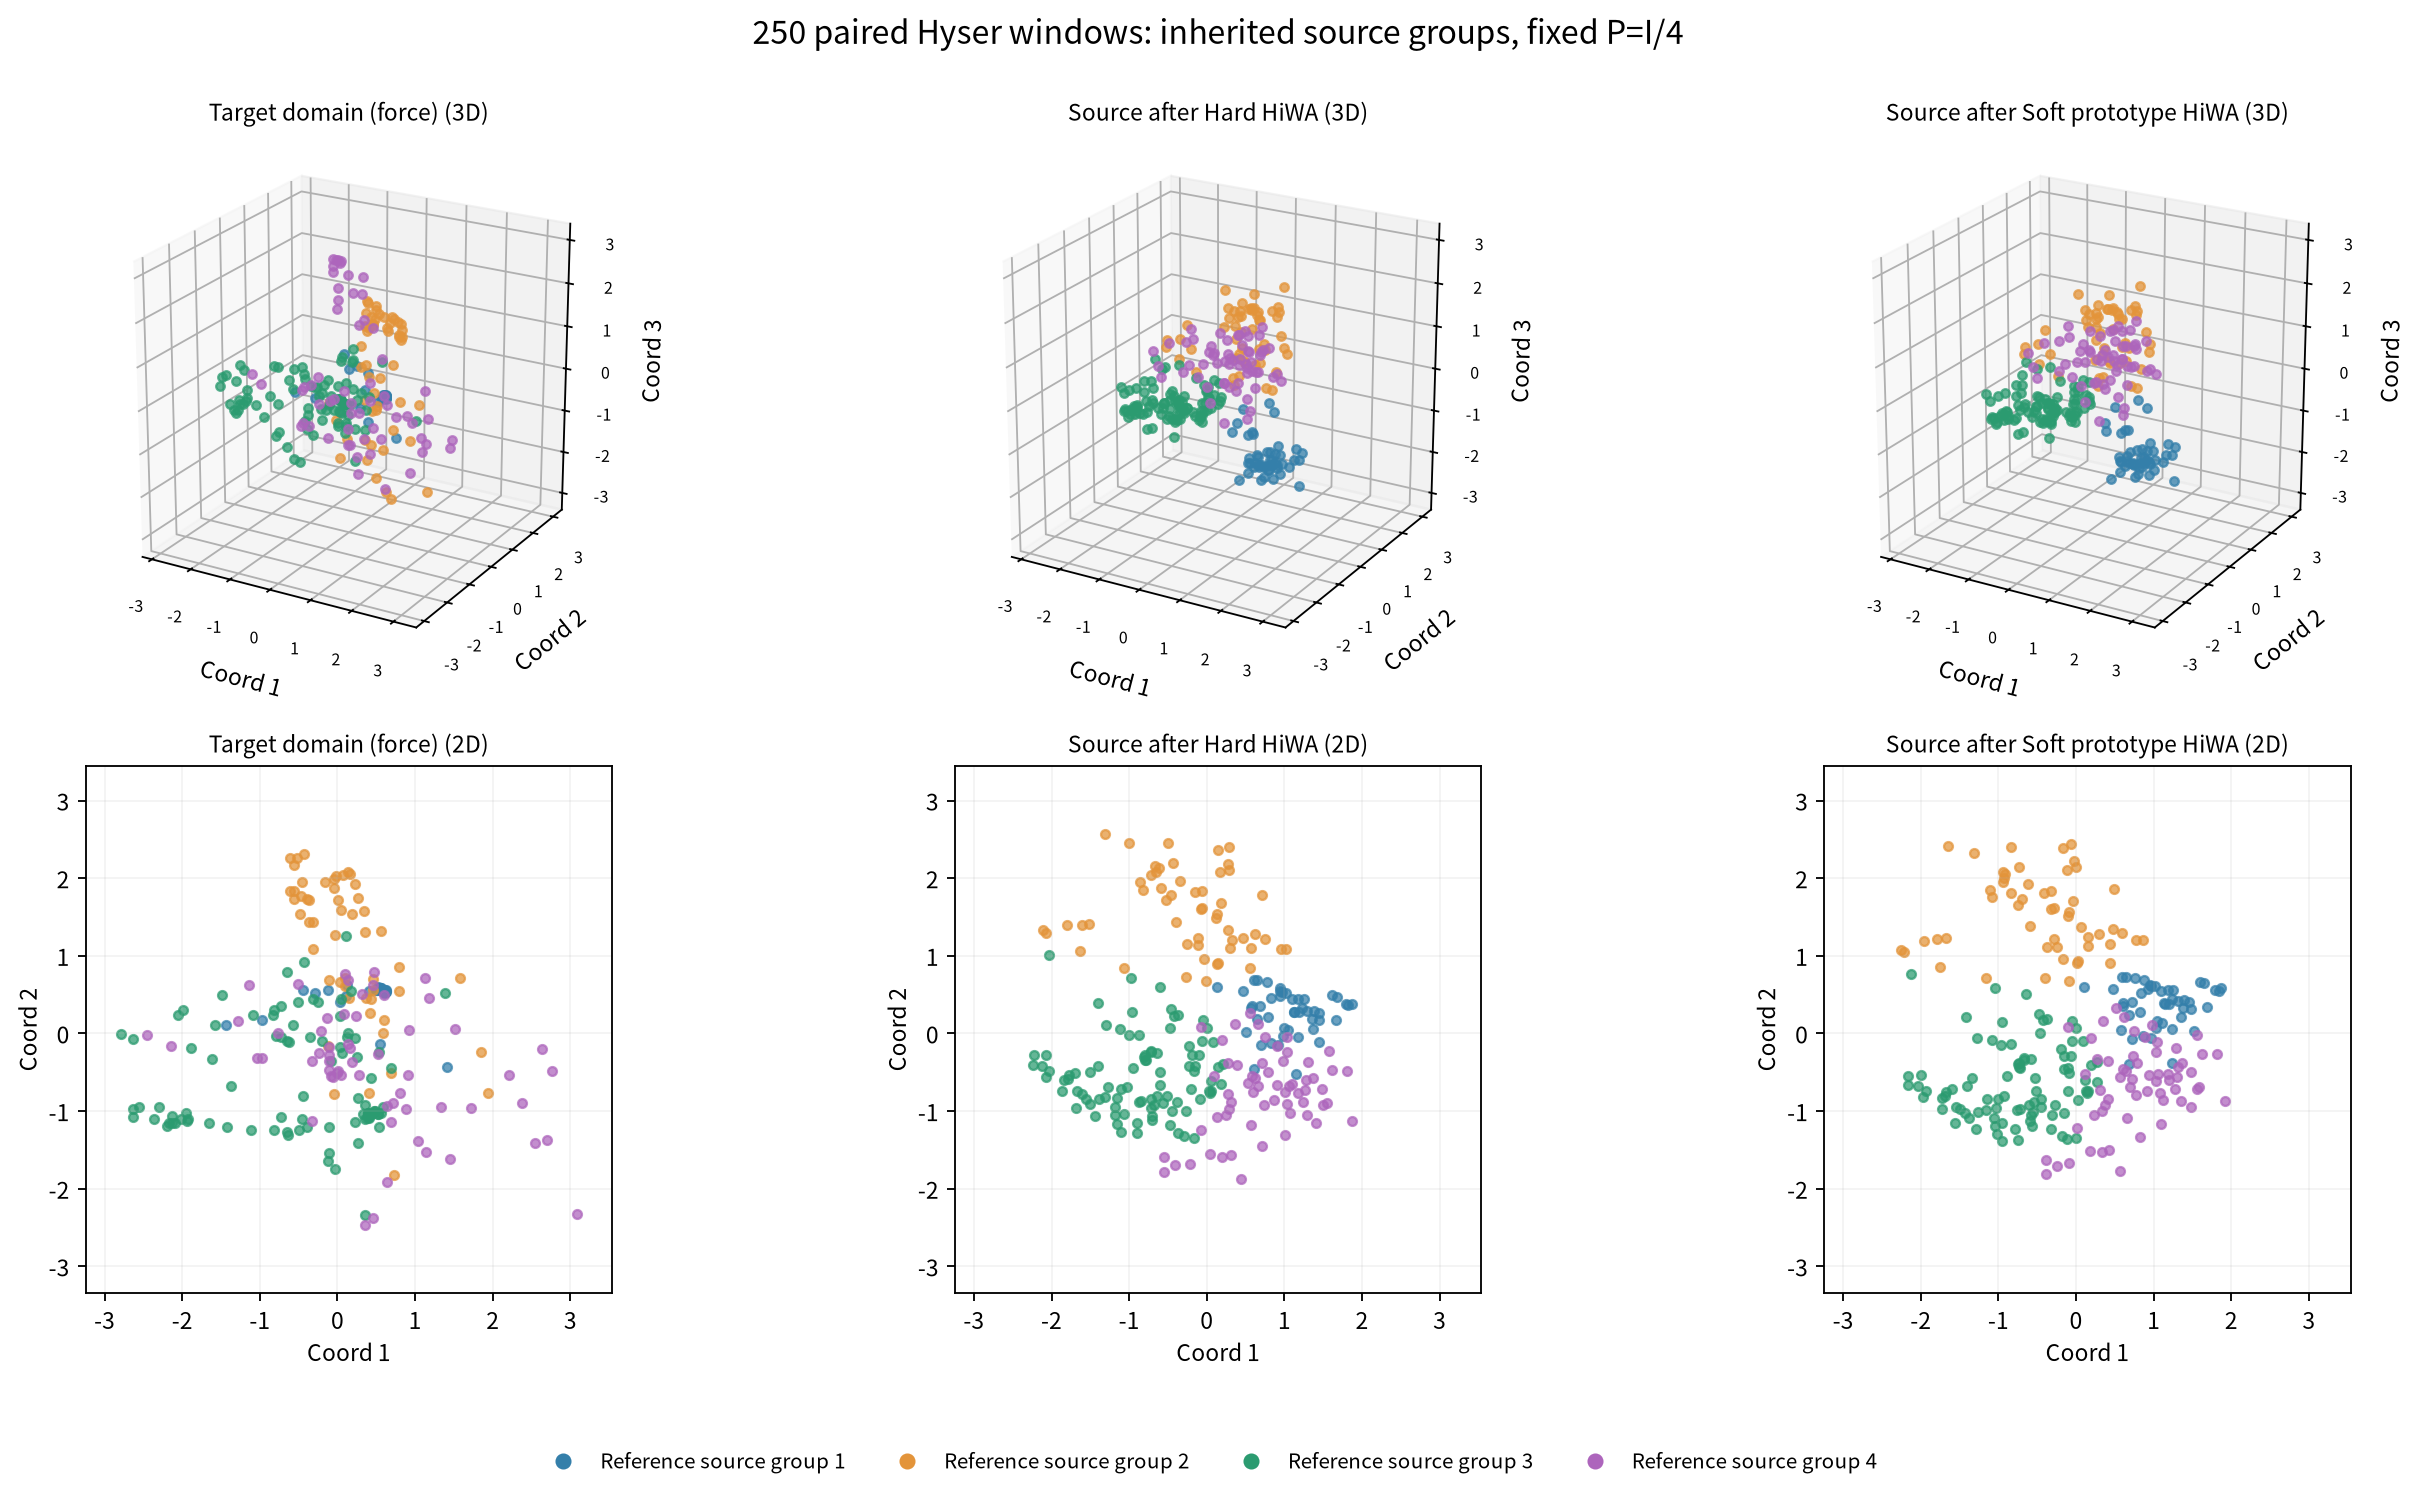
\includegraphics[width=.98\textwidth,height=.74\textheight,keepaspectratio]{figures/05_hard_vs_soft_paired_2d3d.png}
\end{center}
\noindent\small
上排三维、下排二维；左侧是目标力量域，中间是Hard对齐后源域，
右侧是软原型对齐后源域。颜色均使用原源域K-means参考组；
软模型实际使用的是完整概率隶属度，并非图中显示的硬参考组。
图形坐标经过可视化量化，数值表基于全精度原始数据。\normalsize

\clearpage
\section{软隶属度与自由组OT的反例}
\begin{center}
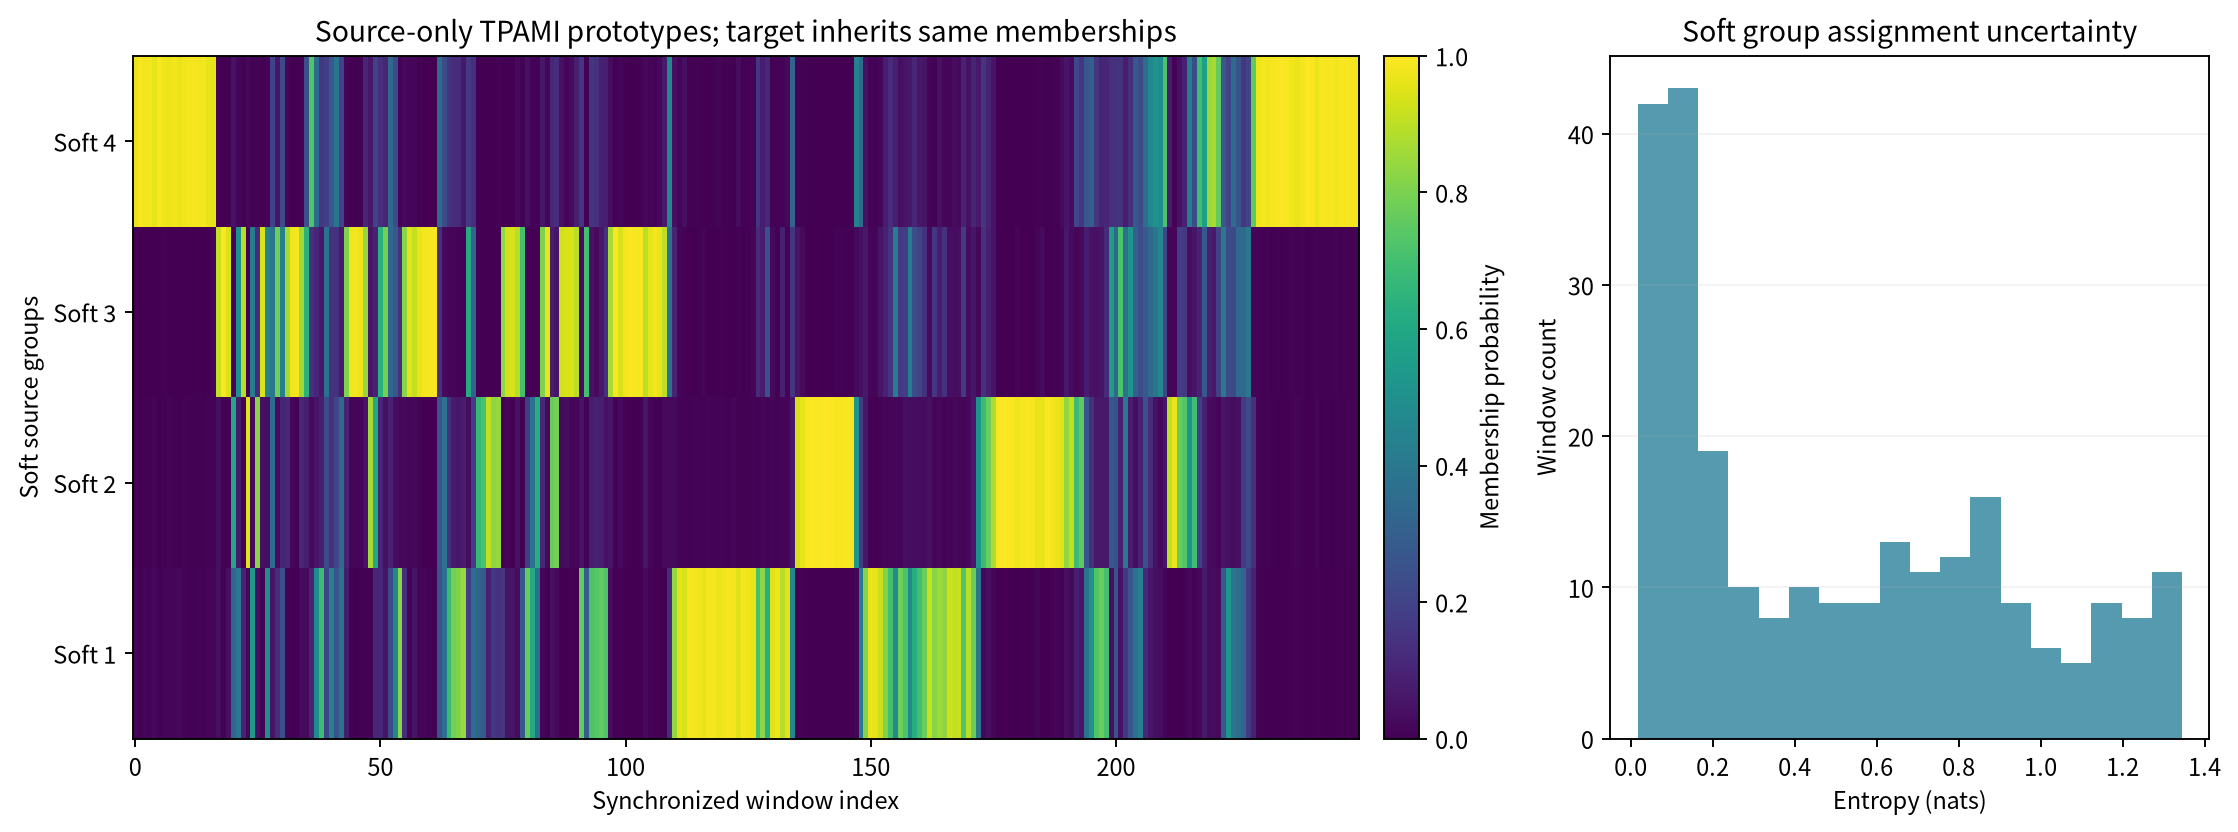
\includegraphics[width=.98\textwidth,height=.41\textheight,keepaspectratio]{figures/06_soft_source_membership.png}
\end{center}
源域软原型的平均隶属熵为$0.50027$ nat，平均最大隶属概率为$0.81484$；
它不是简单地更改硬簇编号。

若不固定已知组对应、允许组级传输$P$自由变化，使用$\mu=0.005$：
Soft-K-means（$\tau=0.5$）的$R^2=-0.16348$、局部共识残差$1.0961$；
Soft原型的$R^2=-0.64435$、局部共识残差$0.4371$。
两者仅达到作者式旋转变化停止阈值，未满足严格ADMM共识残差；
Soft原型的$P$还发生了组错配。\textbf{所以不能认为自由组GCOT必然优于Hard HiWA。}

这250点全部用于同一试次的拟合内评价，且目标分组继承使用了真实时间配对。
数值来自对用户GCOT源码公式的本地移植而非直接导入原仓库文件；
尚不能据此给出无监督跨试次泛化的结论。

\end{document}
